\documentclass[a4paper]{article}

% \usepackage{fullpage}
\usepackage[margin=2.0cm]{geometry}

\usepackage[T1]{fontenc}
\usepackage[english]{babel}
\usepackage{textcomp}
\usepackage{multirow}
\usepackage{float}
\usepackage{fancyhdr}
\usepackage{pdfpages}
\usepackage{longtable}
\usepackage{fancyref}

\usepackage{hyperref}
\hypersetup{
	pdfauthor = {Christian Wemstad},
	pdftitle = {eh2730: Requirements Specifications for ACME Power Company},
	pdfsubject = {EH2730},
	pdfkeywords = {URD, Requirements},
	pdfcreator = {LaTeX with hyperref package},
	pdfproducer = {latex}
}

\usepackage{graphicx}
\usepackage{amsmath}


\title{Assignment II: Requirements Specifications for ACME Power Company}
\author{Henrik Sohlberg <\href{mailto:hsoh@kth.se}{hsoh@kth.se}> %
\and Christian Wemstad <\href{mailto:wemstad@kth.se}{wemstad@kth.se}> %
}

\fancyhf{}
\fancyhead[LE,RO]{\slshape \rightmark}
\fancyhead[LO,RE]{\slshape \leftmark}
\fancyfoot[C]{\thepage}

\begin{document}
\thispagestyle{empty}
\maketitle
\thispagestyle{empty}
\pagestyle{empty}
\newpage
\section*{Version table}
\label{sec:version_tabel}
\begin{table}[H]
	\centering
	\begin{tabular}{|l|l|l|l|}
		\hline
			\textbf{Version} & \textbf{Change log} & \textbf{User} & \textbf{Date}\\
		\hline
		     v. 1 & First version & Mr. Wemstad and Mr. Sohlberg & \today \\
		\hline
	\end{tabular}
\end{table}
\newpage       
\tableofcontents
\newpage
\pagestyle{fancy}
\setcounter{page}{1}

\section{Introduction}
\label{sec:introduction}
\subsection{Purpose and background}
\label{purpose_and_background}
This document is a project plan for the procurement project of ''The ACME WOMS project''. The ''The ACME WOMS project'' project will, if executed, implement a new digital system in the current ACME system collection. This system will be a Work Order Management System (WOMS) targeted to optimize proactive/reactive maintenance and the customer support process, in terms of costs and efficiency.

The background for this procurement project is that the company, ACME, has an outstanding economic issue, which has been a problem the company for a long time. The company has located a low profitability, which they think is an indicator that there may be sub-optimal solutions within the company. ACME has also analyzed the costs of the company and located that one of the biggest cost expenses are the customer support team. Furthermore, recently a new legislation was taken in action enacting a penalty fee for outages longer than 12, increasing the pressure to an already strained budget . The management department believes that cost reductions can be made in the maintenance and repair section if a better control system would be present. \cite{appendixA}

\subsubsection{Vision Statement}
\label{vision_statement}
For ACME who deliver electrical power to factories and households, where the main costs are maintenance and customer support, the WOMS, a COTS software integrated with other systems in the organization, will enhance how proactive and reactive maintenance is functioning and how information can be provided to customers.

Unlike existing work procedures that do not offer the ability to control neither how to dispatch work orders nor to follow up and reduce costs related to maintenance work, the WOMS product will fulfill not only how to control and optimize the maintenance function, but also enable ACME's customer support to provide better and more up-to-date information to customers. 

\subsection{Goals}
The main costs of ACME's business are maintenance, repair and construction and the survey (section \ref{purpose_and_background}) indicates those costs to be beyond industry average. The major goal of this project is to resolve this issue, lower the costs to industry average, increasing the competitive value of the ACME company. Within the same scope, another goal is to tackle the ''12 hour outage penalty'' issue by cutting the costs for this post in half.

Another major cost can be found in the customer care division. A WOMS can support this process, providing function and service to improvement and optimization \cite{appendixB}. Therefore, two goals will be lowering: the number of incoming ''customer complaining cases'', and the average spent time for a customer care employee on an average case.

All the goals is summarized in the table \ref{table:goals}. The goals will be compared to economic report for the time period January 1st 2012 to December 31st 2012.
\begin{center}
	\begin{longtable}{|l|p{3.5cm}|p{3.5cm}|l|}
		\caption{Goals}
		\label{table:goals}\\
		\hline
		\textbf{ID} & \textbf{Description} & \textbf{How} & \textbf{Due Date} \\
		\hline
		\endfirsthead

		\multicolumn{4}{c}%
		{\tablename\ \thetable\ -- \textit{Continued from previous page}} \\
		\hline
		\textbf{ID} & \textbf{Description} & \textbf{How} & \textbf{Due Date} \\
		\hline
		\endhead

		\hline \multicolumn{4}{r}{\textit{Continued on next page}} \\
		\endfoot

		\hline
		\endlastfoot
		%
		GOAL-1 \label{goal-1} & 
		Reduce the expenses for the maintenance, repair, and construction post to < 100\% of industry average &
		By the support of WOMS functionality, improve proactive and reactive maintenance processes &
		May 1st 2016 \\
		\hline
		%
		GOAL-2 \label{goal-2}&
		Lower the costs for ''12 hour outage penalty'' cases by 50\% &
		Embracing prioritized and efficient dispatching of work orders &
		May 1st 2015 \\
		\hline
		%
		GOAL-3 \label{goal-3}&
		A 30\% decrease of costs for the customer care team division &
		Improve the ''outage/service information'' process and quality &
		May 1st 2016 \\
		\hline
		% 
		GOAL-4 \label{goal-4}&
		Replace 20\% of the manual process with automated within the customer care team &
		WOMS will be the key to enable future project or changes to automate this process &
		May 1st 2015 \\
		\hline
		%
	\end{longtable}
\end{center}

\subsection{Document Overview and Conventions}
Section \ref{sec:introduction} is suitable for any stakeholder to read as it is introduction for the whole product and its context.	

Section \ref{sec:overall_description} is an overall description for the product, its users, dependencies, and constraints. Managers of any department is recommended to read this to get a deeper understanding of the procurement product. Direct users will also benefit from reading 2.3 as it concern their tasks and environment.

Section \ref{sec:functional_requirements}

Section \ref{sec:external_interface_requirements}

Section \ref{sec:quality_attributes} is suitable for the IS/IT department. It describes all the 

\subsection{Glossary}
\begin{center}
	\begin{longtable}{|l|l|}
		\caption{Glossary}
		\label{table:glossary}\\
		\hline
		\textbf{Term} & \textbf{Definition}\\
		\hline
		\endfirsthead

		\multicolumn{2}{c}%
		{\tablename\ \thetable\ -- \textit{Continued from previous page}} \\
		\hline
		\textbf{Term} & \textbf{Definition}\\
		\hline
		\endhead

		\hline \multicolumn{2}{r}{\textit{Continued on next page}} \\
		\endfoot

		\hline
		\endlastfoot
		ACC 	& 	The stakeholder \emph{Accounting Team} \\
		\hline
		CC 		& 	The stakeholder \emph{Call Centre Team} \\
		\hline
		CIS 	& 	Customer Information System \\
		\hline
		DMS 	&	Distribution Management System \\
		\hline
		ERP 	& 	Enterprise Resource Planning \\
		\hline
		FT 	& 	The stakeholder \emph{Field Technicians}. Also known as \emph{sub-contractors} \\
		\hline
		M/E 	& 	The stakeholder \emph{Maintenance \& Expansion Team} \\
		\hline
		MO 	& 	The stakeholder \emph{Monitoring Team} \\
		\hline
		NIS 	& 	Network Information System \\
		\hline
		PU 	& 	The stakeholder \emph{Purchasing Team} \\
		\hline
		PDA	& 	Personal Digital Assistant \\
		\hline
		WO 	& 	Work Order \\
		\hline 
		IP address	&	Internet Protocol address \\ 
		\hline
	\end{longtable}
\end{center}

%\clearpage

\section{Overall Description}
\label{sec:overall_description}
\subsection{Product Overview}
The project in hand will be a WOMS, work order management system.  The purpose of this system will be to handle work orders, for maintenance and repair. The system will dispatch work orders to the appropriate field technician, depending on the technicians schedule, location and competence. The system will also have capability to prioritize  work orders  making the currently  most important work executed first.  

\subsection{Product Stakeholders and Users}
\label{sec:produt_stakeholders_and_users}
The product stakeholders have been identified and described in a Stakeholder Profile and a Stakeholder Categorization, see Appendix A to view the models. Furthermore, an Actor Table describing the users, their roles and responsibilities in the system context, can be found in table blabla. As one can see, the table shows the different roles direct users (internal and external stakeholders) enact when interacting with the system, and also what actor roles current systems will have. 
\subsection{Product Environment}
\label{sec:product_environment}
\subsubsection{Planning Maintenance Work}
\label{sec:bp1}
The maintenance work is a large cost driver for ACME, as stated in the background and in Assignment 1 \cite{ass1}, and to be able to fulfill the business goal GOAL-1 - maintenance work is one process that needs to be improved and increased in efficiency. The \textbf{Planning Maintenance Work} process seeks to satisfy these needs. 

In this process, the stakeholders M/E together with the ACC are the main players. M/E analyze the different systems and existing equipment to identify maintenance work to be done. This includes browsing through information, such as how old a system/equipment is, giving indicators to maintenance needs. If M/E locate such necessity, they project a plan and handing it over to ACC who evaluate the plan and its constituents. ACC may find ways to reduce the costs of the plan, e.g. how spare parts will be bought, and finally decide whether it is valuable and motivated to send the plan as a request to PU - to have them sign it.

The WOMS shall support this process by offer new data to M/E in their ''Analyze'' activity, e.g. fail-tendencies for different machineries. It shall also support the ''Project a plan'' activity in a similar way as it will provide data, e.g. statistics of how much time is spent maintaining certain systems/equipment, materials that is usually needed and so on, to make it easier to project better plans.
%
\subsubsection{Creating Work Orders}
\label{sec:bp2}
The \textbf{Creating work orders} process focuses on the way ACME handles work orders. ACME has of today no standardized way of handling work orders. This leads to work orders gets lost and don't get executed even when the were suppose to. In some cases the opposite happens, work orders that the purchasing team thing is too expensive gets executed because they were not consulted before the work order was executed. This process that both make it clear for the company how they should handle their work orders is in the biggest of needs. This process will help the achieving GOAL-1, since no unnecessarily expensive work orders will be executed. The process will also help in solving GOAL-2 since no necessary work orders now will be forgotten. 

In this process there are 3 different main users, MO, M/E and CC. This users have in earlier processes decided that a maintenance/repair/construction work is needed and want to create a work order. This work order then get automatically updated by the NIS to include all the relevant information about the components and other parts in the planned work order. The work order is then handled by the ERP as a new service where an automatic cost calculation is made. The PU will now read the calculations made by the ERP and they will have the final decision on whether or not to execute the work order, this is not done in the WOMS. The final decision is then delivered to the user specifying it in the first place.

A WOMS will help in this process by being a center hub between all the different components in this process. To do this the WOMS needs to be able to transfer data between different systems and have working interfaces for all of these. All the different stakeholders needs to have the an interface that makes it possible for them to create and modify work orders, depending on their work title, which will be stored in the WOMS.
%
\subsubsection{Dispatching Maintenance/Repair Work to Technicians}
\label{sec:bp3}
The \textbf{Dispatching maintenance/repair work to technicians} is triggered when there is a created and approved work order, a result from the business process \ref{creating_work_orders}. To be able to dispatch work orders in a efficient way will contribute to GOALS-1 and GOALS-2, a reason to this is (for example): when a system or equipment is down (broken), the cost is not only the repair cost itself but also the longer an object is out, the higher the costs will be.

This process begins with - a work order operator (may be M/E or MO) has work orders to dispatch. Information such as the work order's priority, the skills and material needed helps the operator in the process of assigning the work order to a FT. Profiles of field technicians is also available including information such as their geographic position and their competence. Before a work order may be dispatched, the operator sends a request to FT who subsequently respond with an accept or deny. If it was accepted, a work order has been dispatched and this business process ends.

WOMS is the underlying system which enables this process to be executed as recently described. Work order operators works directly with WOMS, viewing WO's and FT's profiles and using the system to interact with FT's. WOMS support the FT's activities as it feeds them with request and work orders, and also receives their responds to requests.
\subsubsection{Carry Out Maintenance/Repair Work}
\label{sec:bp4}
\textbf{Carry Out Maintenance/Repair Work} affects the business goals GOAL-1, GOAL-2, and GOAL-3. GOALS-1 and GOALS-2 is pretty straightforward connected to this process, as how ACME and FT's carries out and executes work orders directly affects maintenance/repair/construction costs. We will see that costs within the CC division also are \textbf{indirectly} affected.

Figure \ref{fig:bp4} shows the start of the process. A FT has been assigned and is about to carry out a WO, thereby FT changes the status of the WO to \emph{ACTIVE}. He or she may also obtain information related to the WO, e.g. manuals. Next step is that FT estimates the time to completion for the current WO and shall also, anytime, during the maintenance work update the estimated time. Having this value to be as correct as possible increases the value of the customer care function (where customer contacts to get answers and information of e.g. an outage) - the more accurate information they have access to, the more satisfied customers will be. At last, when a WO is completed, FT shall report time and material used for the recent work. This information is used in other processes, e.g. \ref{sec:bp1} and \ref{sec:bp6}, and is also subject to a cost report entered in ERP system.

WOMS will support this, first of all since it will be the system which enables the information flow within the process. FT's get the WO itself and its information from WOMS via their PDA. They also, via their PDA, send information to WOMS which stores the information (such as a WO's status, time-material reports). WOMS will also act as the ''forwarder'' of the cost report, sending it to ERP.
%
%
%
%
\subsubsection{Inform About Outages and Their Status}
\label{bp5}
An important function in the ACME business is the relationship to their existing customers. Providing customer utility means not only deliver a good product, in this context $\rightarrow$ electrical power, but also nurture the customer in terms of support. According to Appendix A \cite{appendixA}, \emph{''... the second largest share of calls concern outages.''}, hence the importance of this process, connected to GOALS-3 and GOALS-4, is of no doubt. 

Figure \ref{fig:bp5} illustrates this process. Three stakeholders - M/E, MO, and FT - are providers of information concerning outages and their status. CC is the consumers of this information, and need to access it on customer demands. This data is located in the CIS.

The WOMS will support this system as it will function as a man-in-the-middle system, with its purpose to greatly increase the quality of the outage information stored in CIS. As of today, this information is rarely completely updated \cite{appendixA}, a fact WOMS will extinguish. WOMS shall continuously update this information in CIS and as described in \ref{sec:bp4}, where FTs could update this information in real-time, the status of an outage will always be up to date. 

\subsubsection{Analyze Cost and Repair Data}
\label{bp6}
The process of analyzing costs and repair data consequently is a precondition to be able to come up with new solutions and improvement for routines and procedures. These are causes leading to fulfill GOAL-1 and GOAL-2. 

The stakeholder ACC begins gathering information concerning costs originating from maintenance/repair/construction work, e.g. differences in costs that different contractors (FTs) accounts for similar work orders/services.  Next step is to analyze the collected data, resulting in perhaps (to continue with the aforementioned example) valuable knowledge of which contractors that shall be hired in the future and which are not. 

WOMS supports this process by, simple, offer several types of statistics related to work orders. Such data is gathered by the system as we saw in process \ref{sec:bp4}. Today, this functionality is not provided by any system within ACME.
\subsection{Product Functions}

\subsection{Assumption and Dependencies}
\label{sec:assumption_and_dependencies}
The product WOMS specified in this document, with all of its requirements, is dependent on the ACME's current systems functionality. If, for example, there is no system like NIS where network equipment data is stored, WOMS will not be able to fulfill certain requirements - they depend of the functionality of a system like NIS. Same applies for other systems. 

To manage meeting GOAL-4, this procurement project is dependent on future project which we assume will be executed. The WOMS product itself will not be the reason this goal will be fulfilled. However, procuring and installing this WOMS will set preconditions for this change to take place.

\subsection{Design and Implementation Constraints}
\label{sec:desing_and_implementation_constraints}
In the table \ref{table:design_and_implementation_constraints}, design and implementation constraints affecting the implementation of WOMS are presented, extracted from Appendix A \cite{appendixA}.
\begin{center}
	\begin{longtable}{|l|p{5cm}|p{5cm}|}
		\caption{Design and implementation constraints}
		\label{table:design_and_implementation_constraints}\\
		\hline
		\textbf{ID} & \textbf{Constraint} & \textbf{Comment}\\
		\hline
		\endfirsthead

		\multicolumn{3}{c}%
		{\tablename\ \thetable\ -- \textit{Continued from previous page}} \\
		\hline
		\textbf{ID} & \textbf{Constraint} & \textbf{Comment}\\
		\hline
		\endhead

		\hline \multicolumn{3}{r}{\textit{Continued on next page}} \\
		\endfoot
		\hline
		\endlastfoot
		\hline
		2.6.1 & Apply open standards whenever possible & Concerns all ACME's system architecture \\
		\hline
		2.6.2 & Data flow from ACME computers to and from other networks shall pass through ACME's network boundary firewall proxy &
		See section \ref{sec:external_interface_requirements} for more information \\
		\hline
		2.6.3 & No modifications shall be done on the ERP system & WOMS must adapt to the ERP system \\ 
		\hline
	\end{longtable}
\end{center}
%\clearpage

\section{Functional requirements}
\label{sec:functional_requirements}

In this section, the functional requirements connected to each of the business processes listed in section \ref{sec:product_environment}. These functional requirements describe actions of the system, meaning what the system has to do or what functional needs the users will have when interacting with the WOMS. These requirements are prioritized according to the MoSCoW-model. 

\subsection{Planning Maintenance Work}
\label{sub:planning_maintenance_work}
In this section all the functional requirements connected to the business process \textbf{Planning Maintenance Work}, explained in section \ref{sec:bp1}, are listed. As stated in section \ref{sec:bp1}, these requirements are connected to the goal GOAL-1. The ID uniquely identifies the requirements in the format FR-PMW-\{number\}, where  FR stands for functional requirement and PMW stands for planning maintenance work. 


\begin{center}
\begin{longtable}{|c|p{4cm}|p{4cm}|c|c|}
\caption{Software interfaces requirements}
\label{table:software_interfaces}\\
\hline
\textbf{ID}& \textbf{Description} & \textbf{Comment} & \textbf{Priority} & \textbf{Dependencies} \\
\hline
\endfirsthead

\multicolumn{5}{c}%
{\tablename\ \thetable\ -- \textit{Continued from previous page}} \\
\hline
\textbf{ID}& \textbf{Description} & \textbf{Comment} & \textbf{Priority} & \textbf{Dependencies} \\
\hline
\endhead

\hline \multicolumn{5}{r}{\textit{Continued on next page}} \\
\endfoot

\hline
\endlastfoot

\hline
FR-PMW-1 &A M/E user shall access every work orders that have been performed on a specified system equipment. & & Must & -\\
\hline
FR-PMW-2 &A M/E user shall access the time  past since the maintenance/repair/construction work has been performed on a specified system equipment.  & & Must & - \\
\hline
FR-PMW-3 &A M/E user shall access the age on a specified system equipment. & & Must & - \\
\hline
FR-PMW-4 &A M/E user shall be able to see a WO's total execution time.  & & Must & - \\
\hline
FR-PMW-5 &A M/E user shall be able to see which spare parts were used to complete a WO. & & Must & - \\
\hline
FR-PMW-6 &A M/E user shall be able to view what sub-contractor executed a WO. & & Should & - \\
\hline
FR-PMW-7 &A M/E user shall be able to view the difference between estimated execution time and actual execution time on a WO. & & Should & - \\
\hline
FR-PMW-8 &A M/E user shall be able to view similar WO to a selected WO based on location & & Should & - \\
\hline
FR-PMW-9 &A M/E user shall be able to view similar WO to a selected WO based on type of error & & Should & - \\
\hline

\end{longtable}
\end{center}


\subsection{Creating a Work Order}
\label{sub:creating_a_work_order}
In this section all the functional requirements connected to the business process \textbf{Creating a Work Order}, explained in section \ref{sec:bp2}, are listed. As stated in section \ref{sec:bp2}, these requirements are connected to the goals GOAL-1 and GOAL-2. The ID uniquely identifies the requirements in the format FR-CWO-\{number\}, where  FR stands for functional requirement and CWO stands for creating work order. 


\begin{center}
\begin{longtable}{|c|p{4cm}|p{4cm}|c|c|}
\caption{Creating a work order requirements}
\label{table:creating_a_work_order}\\
\hline
\textbf{ID}& \textbf{Description} & \textbf{Comment} & \textbf{Priority} & \textbf{Dependencies} \\
\hline
\endfirsthead

\multicolumn{5}{c}%
{\tablename\ \thetable\ -- \textit{Continued from previous page}} \\
\hline
\textbf{ID}& \textbf{Description} & \textbf{Comment} & \textbf{Priority} & \textbf{Dependencies} \\
\hline
\endhead

\hline \multicolumn{5}{r}{\textit{Continued on next page}} \\
\endfoot

\hline
\endlastfoot

\hline

FR-CWO-1 & A user shall be able to create a new  WO.& A user is either a MO, M/E or CC. & Must & - \\
\hline
FR-CWO-2 & A user shall be able to prioritize a WO. & A user is either a MO, M/E or CC.& Must & FR-CWO-1\\
\hline
FR-CWO-3 & A user shall be able to edit a WO.  & A user is either a MO, M/E or CC user & Must & FR-CWO-1 \\
\hline
FR-CWO-4 & A user shall be able to remove a WO. & A user is either a MO, M/E or CC user & Must & FR-CWO-1 \\
\hline
FR-CWO-5 & The WOMS shall be able gather system equipment manuals from the NIS. & & Must & - \\
\hline
FR-CWO-6 & The WOMS shall be able to link system equipment manuals to WOs. & & Must & FR-CWO-5 \\
\hline
FR-CWO-7 & The WOMS shall be able to order a new service in the ERP system. & & Must & - \\
\hline
FR-CWO-8 & The WOMS shall be able to read a service order response from the ERP system. & & Must & - \\
\hline
FR-CWO-9 & The WOMS shall be able to set a WO as either accepted or denied. & & Must & - \\
\hline
FR-CWO-10& A user shall be able to set a WO as either accepted or denied. &A user is either a MO, M/E or CC user & Must & - \\
\hline

\end{longtable}
\end{center}

\subsection{Dispatching Maintenance/ Repair Work}
\label{sub:dispatching_maintenance}	
In this section all the functional requirements connected to the business process \textbf{Dispatching Maintenance/ Repair Work}, explained in section \ref{sec:bp3}, are listed. As stated in section \ref{sec:bp3}, these requirements are connected to the goals GOAL-1 and GOAL-2. The ID uniquely identifies the requirements in the format FR-CWO-\{number\}, where  FR stands for functional requirement and DM stands for dispatching maintenance. 


\begin{center}
\begin{longtable}{|c|p{4cm}|p{4cm}|c|c|}
\caption{Dispatching maintenance/ repair work requirements}
\label{table:dispatching_maintenance}\\
\hline
\textbf{ID}& \textbf{Description} & \textbf{Comment} & \textbf{Priority} & \textbf{Dependencies} \\
\hline
\endfirsthead

\multicolumn{5}{c}%
{\tablename\ \thetable\ -- \textit{Continued from previous page}} \\
\hline
\textbf{ID}& \textbf{Description} & \textbf{Comment} & \textbf{Priority} & \textbf{Dependencies} \\
\hline
\endhead

\hline \multicolumn{5}{r}{\textit{Continued on next page}} \\
\endfoot

\hline
\endlastfoot

\hline
FR-DM-1	& A user shall be able to view all WOs& & Must & - \\ 
\hline
FR-DM-2	&A user shall be able to sort WOs  on status &Status can either be accepted, active, denied or completed. A user is either a MO or  M/E. & Must & FR-DM-1 \\ 
\hline
FR-DM-3	&A user shall be able to sort WOs  on priority &A user is either a MO or  M/E. & Must & FR-DM-1\\ 
\hline
FR-DM-4	&A user shall be able to view the field technician's competence required to execute a WO. & & Must & - \\ 
\hline
FR-DM-5	&A user shall able to see which spare parts are needed for the work order. & & Must & - \\ 
\hline
FR-DM-6	&A user shall be able to view the location of a work order. & & Must & - \\ 
\hline
FR-DM-7	&A user shall be able to view all available FTs on duty in real time. & & Must & - \\ 
\hline
FR-DM-8	&A user shall be able to view an available FT's competency. & & Must & FR-DM-7\\ 
\hline
FR-DM-9	&A user shall be able to view an available FT's current geographic location. & & Must & FR-DM-7 \\ 
\hline
FR-DM-10&The WOMS shall be able to select the most appropriate FT for a WO. & Most appropriate based on location, competence and work load & Must & - \\
\hline
FR-DM-11&A user shall be able to send a WO request to a FT. & & Must & - \\  
\hline
FR-DM-12&A FT shall be able to respond Yes or No to a WO request. & & Must & - \\ 
\hline
FR-DM-13&A user shall to see the FT's response for a WO request. & & Must & - \\ 
\hline
FR-DM-14&A user shall be able to dispatch a WO to a FT. & & Must & - \\ 
\hline

\end{longtable}
\end{center}


\subsection{Carry Out Maintenance/Repair Work}
\label{sub:carry_out_maintenance}
In this section all the functional requirements connected to the business process \textbf{Carry Out Maintenance/Repair Work}, explained in section \ref{sec:bp4}, are listed. As stated in section \ref{sec:bp4}, these requirements are connected to the goals GOAL-1, GOAL-2, and GOAL-3. The ID uniquely identifies the requirements in the format FR-CWO-\{number\}, where  FR stands for functional requirement and COM stands for carry out maintenance.  



\begin{center}
\begin{longtable}{|c|p{4cm}|p{4cm}|c|c|}
\caption{Carry out maintenance/repair work requirements}
\label{table:carry_out_maintenance}\\
\hline
\textbf{ID}& \textbf{Description} & \textbf{Comment} & \textbf{Priority} & \textbf{Dependencies} \\
\hline
\endfirsthead

\multicolumn{5}{c}%
{\tablename\ \thetable\ -- \textit{Continued from previous page}} \\
\hline
\textbf{ID}& \textbf{Description} & \textbf{Comment} & \textbf{Priority} & \textbf{Dependencies} \\
\hline
\endhead

\hline \multicolumn{5}{r}{\textit{Continued on next page}} \\
\endfoot

\hline
\endlastfoot


FR-COM-1 & A FT shall be able to view a WO, stored in the WOMS. & & Must & - \\ 
\hline
FR-COM-2 & A FT shall be able to change the status of a WO. & & Must & - \\ 
\hline
FR-COM-3 & A FT shall be able to access system equipment information related to the current WO. & & Must & - \\ 
\hline
FR-COM-4 & A FT shall be able to change the status of a WO. & & Must & - \\ 
\hline
FR-COM-5 & A FT shall be able to set the estimated remaining time on a WO. & & Must & - \\ 
\hline
FR-COM-6 & A FT shall be able to set the time spent on a WO. & & Must & - \\ 
\hline
FR-COM-7 & A FT shall be able to store what spare parts were used to execute a WO. & & Must & - \\ 
\hline
FR-COM-8 & The WOMS shall be able to store a cost report connected to a WO. &A cost report contains: Material costs and time costs. & Must & ERI-HI-1 \\ 
\hline
FR-COM-9 & The WOMS shall be able to enter a cost report into the ERP. &A cost report contains: Material costs and time costs. & Must & ERI-HI-1 \\ 
\hline

\end{longtable}
\end{center}


\subsection{Inform About Outages and Their Status}
\label{sub:inform_about_outages}
In this section all the functional requirements connected to the business process \textbf{Inform About Outages and Their Status}, explained in section \ref{sec:bp5}, are listed. As stated in section \ref{sec:bp5}, these requirements are connected to the goals GOAL-3 and GOAL-4. The ID uniquely identifies the requirements in the format FR-CWO-\{number\}, where  FR stands for functional requirement and IAO stands for inform about outages. 


\begin{center}
\begin{longtable}{|c|p{4cm}|p{4cm}|c|c|}
\caption{Inform about outages and their status}
\label{table:inform_about_outages}\\
\hline
\textbf{ID}& \textbf{Description} & \textbf{Comment} & \textbf{Priority} & \textbf{Dependencies} \\
\hline
\endfirsthead

\multicolumn{5}{c}%
{\tablename\ \thetable\ -- \textit{Continued from previous page}} \\
\hline
\textbf{ID}& \textbf{Description} & \textbf{Comment} & \textbf{Priority} & \textbf{Dependencies} \\
\hline
\endhead

\hline \multicolumn{5}{r}{\textit{Continued on next page}} \\
\endfoot

\hline
\endlastfoot

FR-IAO-1 & A user shall be able to view the status of a WO. & A user is either a M/E or MO & Must & - \\ 
\hline
FR-IAO-2 & A user shall be able to view the estimated time to completion on a WO. &  A user is either a M/E or MO & Must & - \\
\hline
FR-IAO-3 & The WOMS shall be able to insert outage statuses in the CIS. & & Must & - \\ 
\hline
FR-IAO-4 & The WOMS shall be able to update outage statuses in the CIS. & & Must & - \\ 
\hline
FR-IAO-5 & The WOMS shall be able to remove outages statuses in the CIS. & & Must & - \\
\hline 
FR-IAO-6 & A FT shall be able to insert outage statuses & & Should & - \\
\hline
FR-IAO-7 & A FT shall be able to update outage statuses & & Should & - \\
\hline
FR-IAO-8 & A FT shall be able to remove outage statuses & & Should & - \\
\hline


\end{longtable}
\end{center}


\subsection{Analyze Cost and Repair Data}
\label{sub:analyze_cost}
In this section all the functional requirements connected to the business process \textbf{Analyze Cost and Repair Data}, explained in section \ref{sec:bp6}, are listed. As stated in section \ref{sec:bp6}, these requirements are connected to the goals GOAL-1 and GOAL-2. The ID uniquely identifies the requirements in the format FR-CWO-\{number\}, where  FR stands for functional requirement and AC stands for analyze cost.


\begin{center}
\begin{longtable}{|c|p{4cm}|p{4cm}|c|c|}
\caption{Analyze cost and repair data}
\label{table:analyze_cost}\\
\hline
\textbf{ID}& \textbf{Description} & \textbf{Comment} & \textbf{Priority} & \textbf{Dependencies} \\
\hline
\endfirsthead

\multicolumn{5}{c}%
{\tablename\ \thetable\ -- \textit{Continued from previous page}} \\
\hline
\textbf{ID}& \textbf{Description} & \textbf{Comment} & \textbf{Priority} & \textbf{Dependencies} \\
\hline
\endhead

\hline \multicolumn{5}{r}{\textit{Continued on next page}} \\
\endfoot

\hline
\endlastfoot

FR-AC-1 &An ACC user shall be able to view what sub-contractor executed a WO. & & Must & - \\
\hline
FR-AC-2 &An ACC user shall be able to view mean execution time for a WO  for each sub-contractor & & Must & - \\
\hline
FR-AC-3 &An ACC user shall be able to view what specific FT executed a WO & & Should & - \\
\hline
FR-AC-4 &An ACC user shall be able to view a cost report connected to a WO. & & Must & - \\
\hline
FR-AC-5 &An ACC user shall be able to view the difference between estimated time and actual executed time. & & Should & - \\
\hline
FR-AC-6 &An ACC user shall be able to view the actual execution time for a WO & & Must & - \\
\hline
FR-AC-7 &An ACC user shall be able to view a similar WO to a selected WO based on location & & Should & - \\
\hline
FR-AC-8 &An ACC user shall be able to view a similar WO to a selected WO based on type of error & & Should & - \\
\hline

\end{longtable}
\end{center}







%\clearpage

\section{External interface requirements}
\label{sec:external_interface_requirements}

To be able to fulfill all of the requirements specified in section 3 some additional requirements for the WOMS has to be specified. These requirements are the \textbf{External interface requirements}, the requirements that specify how the WOMS will interact with other systems and users.  These requirements are separated into 3 different categories, depending on what they describe, \textbf{Software interface requirements}, \textbf{Communications interfaces requirements} and \textbf{Hardware interfaces requirements}. A more in detail description of each of the interfaces are described in their own subchapter, but the main focus can be seen as \textbf{Software interface requirements} is what information will be transmitted, \textbf{Communications interfaces requirements} is what type technical interface the communication will be on and \textbf{Hardware interfaces requirements} will be the hardware the WOMS comes in contact with. 

The requirements in this section is elicited from the Appendix A document \cite{A}, as well as interviews with the IS/IT-department. To get a greater understanding of how the WOMS will, technically, fit in the current ACME IT environment an overview of the communications are present in figure \ref{fig:external_interfaces}


\begin{figure}[H]
	\centering
	\setlength\fboxsep{7pt}
	\setlength\fboxrule{0.5pt}
	\fbox{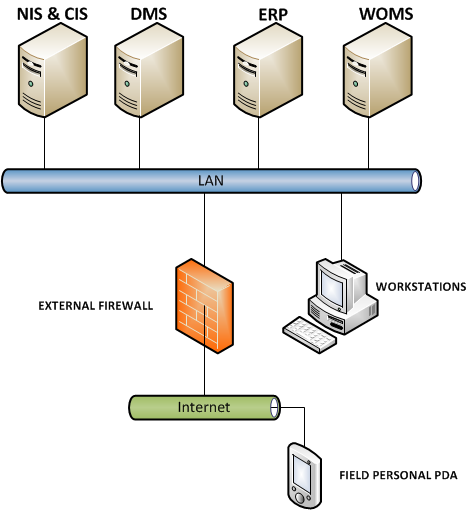
\includegraphics[scale = 0.8]{images/external_interfaces.png}}
	\caption{The external interfaces of the ACME network}
	\label{fig:external_interfaces}                      	
\end{figure}

All of the requirements in this section will be prioritized according to the MosCoW scheme, in the same way as the requirements in section \ref{sec:functional_requirements}.	

NOTE: No requirements on needed changes for other parts of the IT-system are listed here, only requirements that directly affect that WOMS are specified. I.e. there are no requirements on that the PDA needs to be able to connect to the LAN, see fig. \ref{fig:external_interfaces}, only requirements on how the PDA interacts with the WOMS while it's on the LAN.

\subsection{Software interfaces}
\label{sub:software_interfaces}

\textbf{Software interfaces} focuses on the connection the new WOMS will have with other system in the IT environment. Even though figure \ref{fig:external_interfaces} states that the WOMS will act like any other server in the network, the integration between WOMS and the current systems are far greater than the integration between the current systems.  In table \ref{table:software_interfaces} the software interfaces requirements that are needed are listed.

\begin{center}
\begin{longtable}{|l|p{4cm}|p{4cm}|l|l|}
\caption{Software interface requirements}
\label{table:software_interfaces}\\
\hline
\textbf{ID}& \textbf{Description} & \textbf{Comment} & \textbf{Priority} & \textbf{Dependencies}\\
\hline
\endfirsthead

\multicolumn{5}{c}%
{\tablename\ \thetable\ -- \textit{Continued from previous page}} \\
\hline
\textbf{ID}& \textbf{Description} & \textbf{Comment} & \textbf{Priority} & \textbf{Dependencies} \\
\hline
\endhead

\hline \multicolumn{5}{r}{\textit{Continued on next page}} \\
\endfoot

\hline
\endlastfoot

\hline

ERI-SI-1& The WOMS shall access the ERP to read any data & & & \\
\hline
ERI-SI-2& The WOMS shall access the ERP to update any data & & & \\
\hline
ERI-SI-3& The WOMS shall access the ERP to delete any data & & & \\
\hline
ERI-SI-4& The WOMS shall access the NIS to read any data & & & \\
\hline
ERI-SI-5& The WOMS shall access the NIS  to modify any data & & & \\
\hline
ERI-SI-6& The WOMS shall access the NIS  to delete any data & & & \\
\hline

\end{longtable}
\end{center}

\subsection{Communication interfaces}
\label{sub:communication_interfaces}

The current interaction of the systems are based on Ethernet connections, this will therefore be the main way the system connects with other systems in the network. Listed in table \ref{table:communication_interfaces} are all the requirements on the communication interfaces.

\begin{center}
\begin{longtable}{|l|p{4cm}|p{4cm}|l|l|}
\caption{Communication interface requirements}
\label{table:communication_interfaces}\\
\hline
\textbf{ID}& \textbf{Description} & \textbf{Comment} & \textbf{Priority} & \textbf{Dependencies}\\
\hline
\endfirsthead

\multicolumn{5}{c}%
{\tablename\ \thetable\ -- \textit{Continued from previous page}} \\
\hline
\textbf{ID}& \textbf{Description} & \textbf{Comment} & \textbf{Priority} & \textbf{Dependencies} \\
\hline
\endhead

\hline \multicolumn{5}{r}{\textit{Continued on next page}} \\
\endfoot

\hline
\endlastfoot

ERI-CI-1& All communication on the LAN, with the WOMS, shall be on Ethernet. & & Must & \\
\hline
ERI-CI-2& The WOMS only access way to units outside the ACME LAN is through the firewall, via Ethernet. & Units, will be, but are not limited to, PDAs & Must & \\
\hline

\end{longtable}
\end{center}


\subsection{Hardware interfaces}
\label{sub:hardwar_interfaces}

A \textbf{Hardware interfaces} requirement is a requirement specifying what kind of other hardware that will communicate with the WOMS. The WOMS will need to be accessible from both internal workstations, as well as external PDAs, see fig. \ref{fig:functional_requirements}. To achieve this there are some hardware interfaces requirements that needs to be fulfilled:

\begin{center}
\begin{longtable}{|l|p{4cm}|p{4cm}|l|l|}
\caption{Hardware interface requirements}
\label{table:communication_interfaces}\\
\hline
\textbf{ID}& \textbf{Description} & \textbf{Comment} & \textbf{Priority} & \textbf{Dependencies}\\
\hline
\endfirsthead

\multicolumn{5}{c}%
{\tablename\ \thetable\ -- \textit{Continued from previous page}} \\
\hline
\textbf{ID}& \textbf{Description} & \textbf{Comment} & \textbf{Priority} & \textbf{Dependencies} \\
\hline
\endhead

\hline \multicolumn{5}{r}{\textit{Continued on next page}} \\
\endfoot

\hline
\endlastfoot

ERI-HI-1& The WOMS shall exchange data with the all servers on the LAN. & Servers are, the NIS \& CIS server, the DMS server and the ERP server. & Must & \\
\hline
ERI-CI-2& The WOMS shall be accessible from the Field Personal PDAs. & & Must & \\
\hline

\end{longtable}
\end{center} 


%\clearpage

\section{Quality attributes} 
\label{sec:quality_attributes}

This section will handle all of the \textbf{Quality attributes}, also called non-functional attributes.  In difference to section \ref{sec:functional_requirements}-\ref{sec:external_interface_requirements} that describe what the new system shall do, the quality attributes describe how the system shall be. \cite{idi.ntnu}  Quality attributes can i.e. describe uptime requirements, system architecture and security requirements.
Below, the \textbf{Quality attributes} for the WOMS system are listed. The requirements are categorized into security, safety, reliability and availability. The ID for the quality attributes are QA-\{number\}, where QA stands for quality attributes.

\begin{center}
\begin{longtable}{|l|p{4cm}|p{2cm}|l|p{1.5cm}|l|l|}
\caption{Quality attributes}
\label{table:5_requirements}\\
\hline
\textbf{ID}& \textbf{Description} & \textbf{Comment} & \textbf{Category} & \textbf{RBP}&\textbf{Priority} & \textbf{Dependencies}\\
\hline
\endfirsthead

\multicolumn{7}{c}%
{\tablename\ \thetable\ -- \textit{Continued from previous page}} \\
\hline
\textbf{ID}& \textbf{Description} & \textbf{Comment} & \textbf{Category} & \textbf{RBP}&\textbf{Priority} & \textbf{Dependencies}\\
\hline
\endhead

\hline \multicolumn{7}{r}{\textit{Continued on next page}} \\
\endfoot

\hline
\endlastfoot

\hline

QA-1	& The WOMS shall have at least $95\%$ rate of picking the most appropriate field technician & Validated through testing &	Reliability & \ref{sec:bp3}&Must & FR-DM-10\\
\hline
QA-2	& The WOMS shall always dispatch the highest prioritized WO first to field technicians. & Validated through testing & Reliability &\ref{sec:bp3} & Must & \\
\hline
QA-3	& The WOMS shall have an overall uptime of at least $99\%$ each month. & Validated through testing & Availability &\ref{sec:bp1}, \ref{sec:bp2}, \ref{sec:bp3}, \ref{sec:bp4}, \ref{sec:bp5}, \ref{sec:bp6} & Must & \\
\hline
QA-4	& The WOMS shall SQL-parse all input data so harmful inputs will not affect the database & Validated through testing , SQL-parsing means removing all illegal syntax from the text. & Safety &\ref{sec:bp1}, \ref{sec:bp2}, \ref{sec:bp3}, \ref{sec:bp4}, \ref{sec:bp5}, \ref{sec:bp6} & Must & \\
\hline
QA-5	& The WOMS shall only allow 3 authorization attempts from each IP before the IP address is blocked for 15 minutes. & Validated through testing & Security &\ref{sec:bp1}, \ref{sec:bp2}, \ref{sec:bp3}, \ref{sec:bp4}, \ref{sec:bp5}, \ref{sec:bp6} &Must & \\
\hline
QA-6	& The WOMS shall automatically logout a user if inactive, no input, for 15 minutes. & Validated through testing & Security &\ref{sec:bp1}, \ref{sec:bp2}, \ref{sec:bp3}, \ref{sec:bp4}, \ref{sec:bp5}, \ref{sec:bp6} & Must & \\
\hline
QA-7	& The WOMS shall have customizable security settings for each user. & Validated through testing. Settings regarding, if allowed to edit, allowed to read or allowed to delete WOs. & Security & \ref{sec:bp1}, \ref{sec:bp2}, \ref{sec:bp3}, \ref{sec:bp4}, \ref{sec:bp5}, \ref{sec:bp6}&Must & \\
\hline
QA-8	& Connections from outside of the ACME LAN to the WOMS shall be encrypted with TLS 1.2 & Validated through testing. & Security & \ref{sec:bp3}, \ref{sec:bp4}, \ref{sec:bp5}&Must & \\

\end{longtable}
\end{center}




\clearpage

\addcontentsline{toc}{section}{References}
\begin{thebibliography}{99}     
	
%\bibitem{gott2} \emph{Gottesdiener, Ellen. \textsl{"The Software Requirements Memmory Jogger" chapter 2}. GOAL/QPC, 2005}

\bibitem{idi.ntnu} \emph{Eide, Petter L. H. \textsl{"Quantification and Traceability of Requirements"} Gathered 2012-12-09 } <\url{http://www.idi.ntnu.no/grupper/su/fordypningsprosjekt-2005/eide-fordyp05.pdf}>

% \bibitem{projectsmart} \emph{Singh, Manjeet. \textsl{"Rescuing Projects in Crisis: Project Turnaround Pointers"} Gathered 2012-11-20} <\url{http://www.projectsmart.co.uk/rescuing-projects-in-crisis.html}> 

\end{thebibliography}
\clearpage

\appendix
\section{Context Diagram}
\begin{figure}[!h]
	\vspace{1cm}
	\centering
	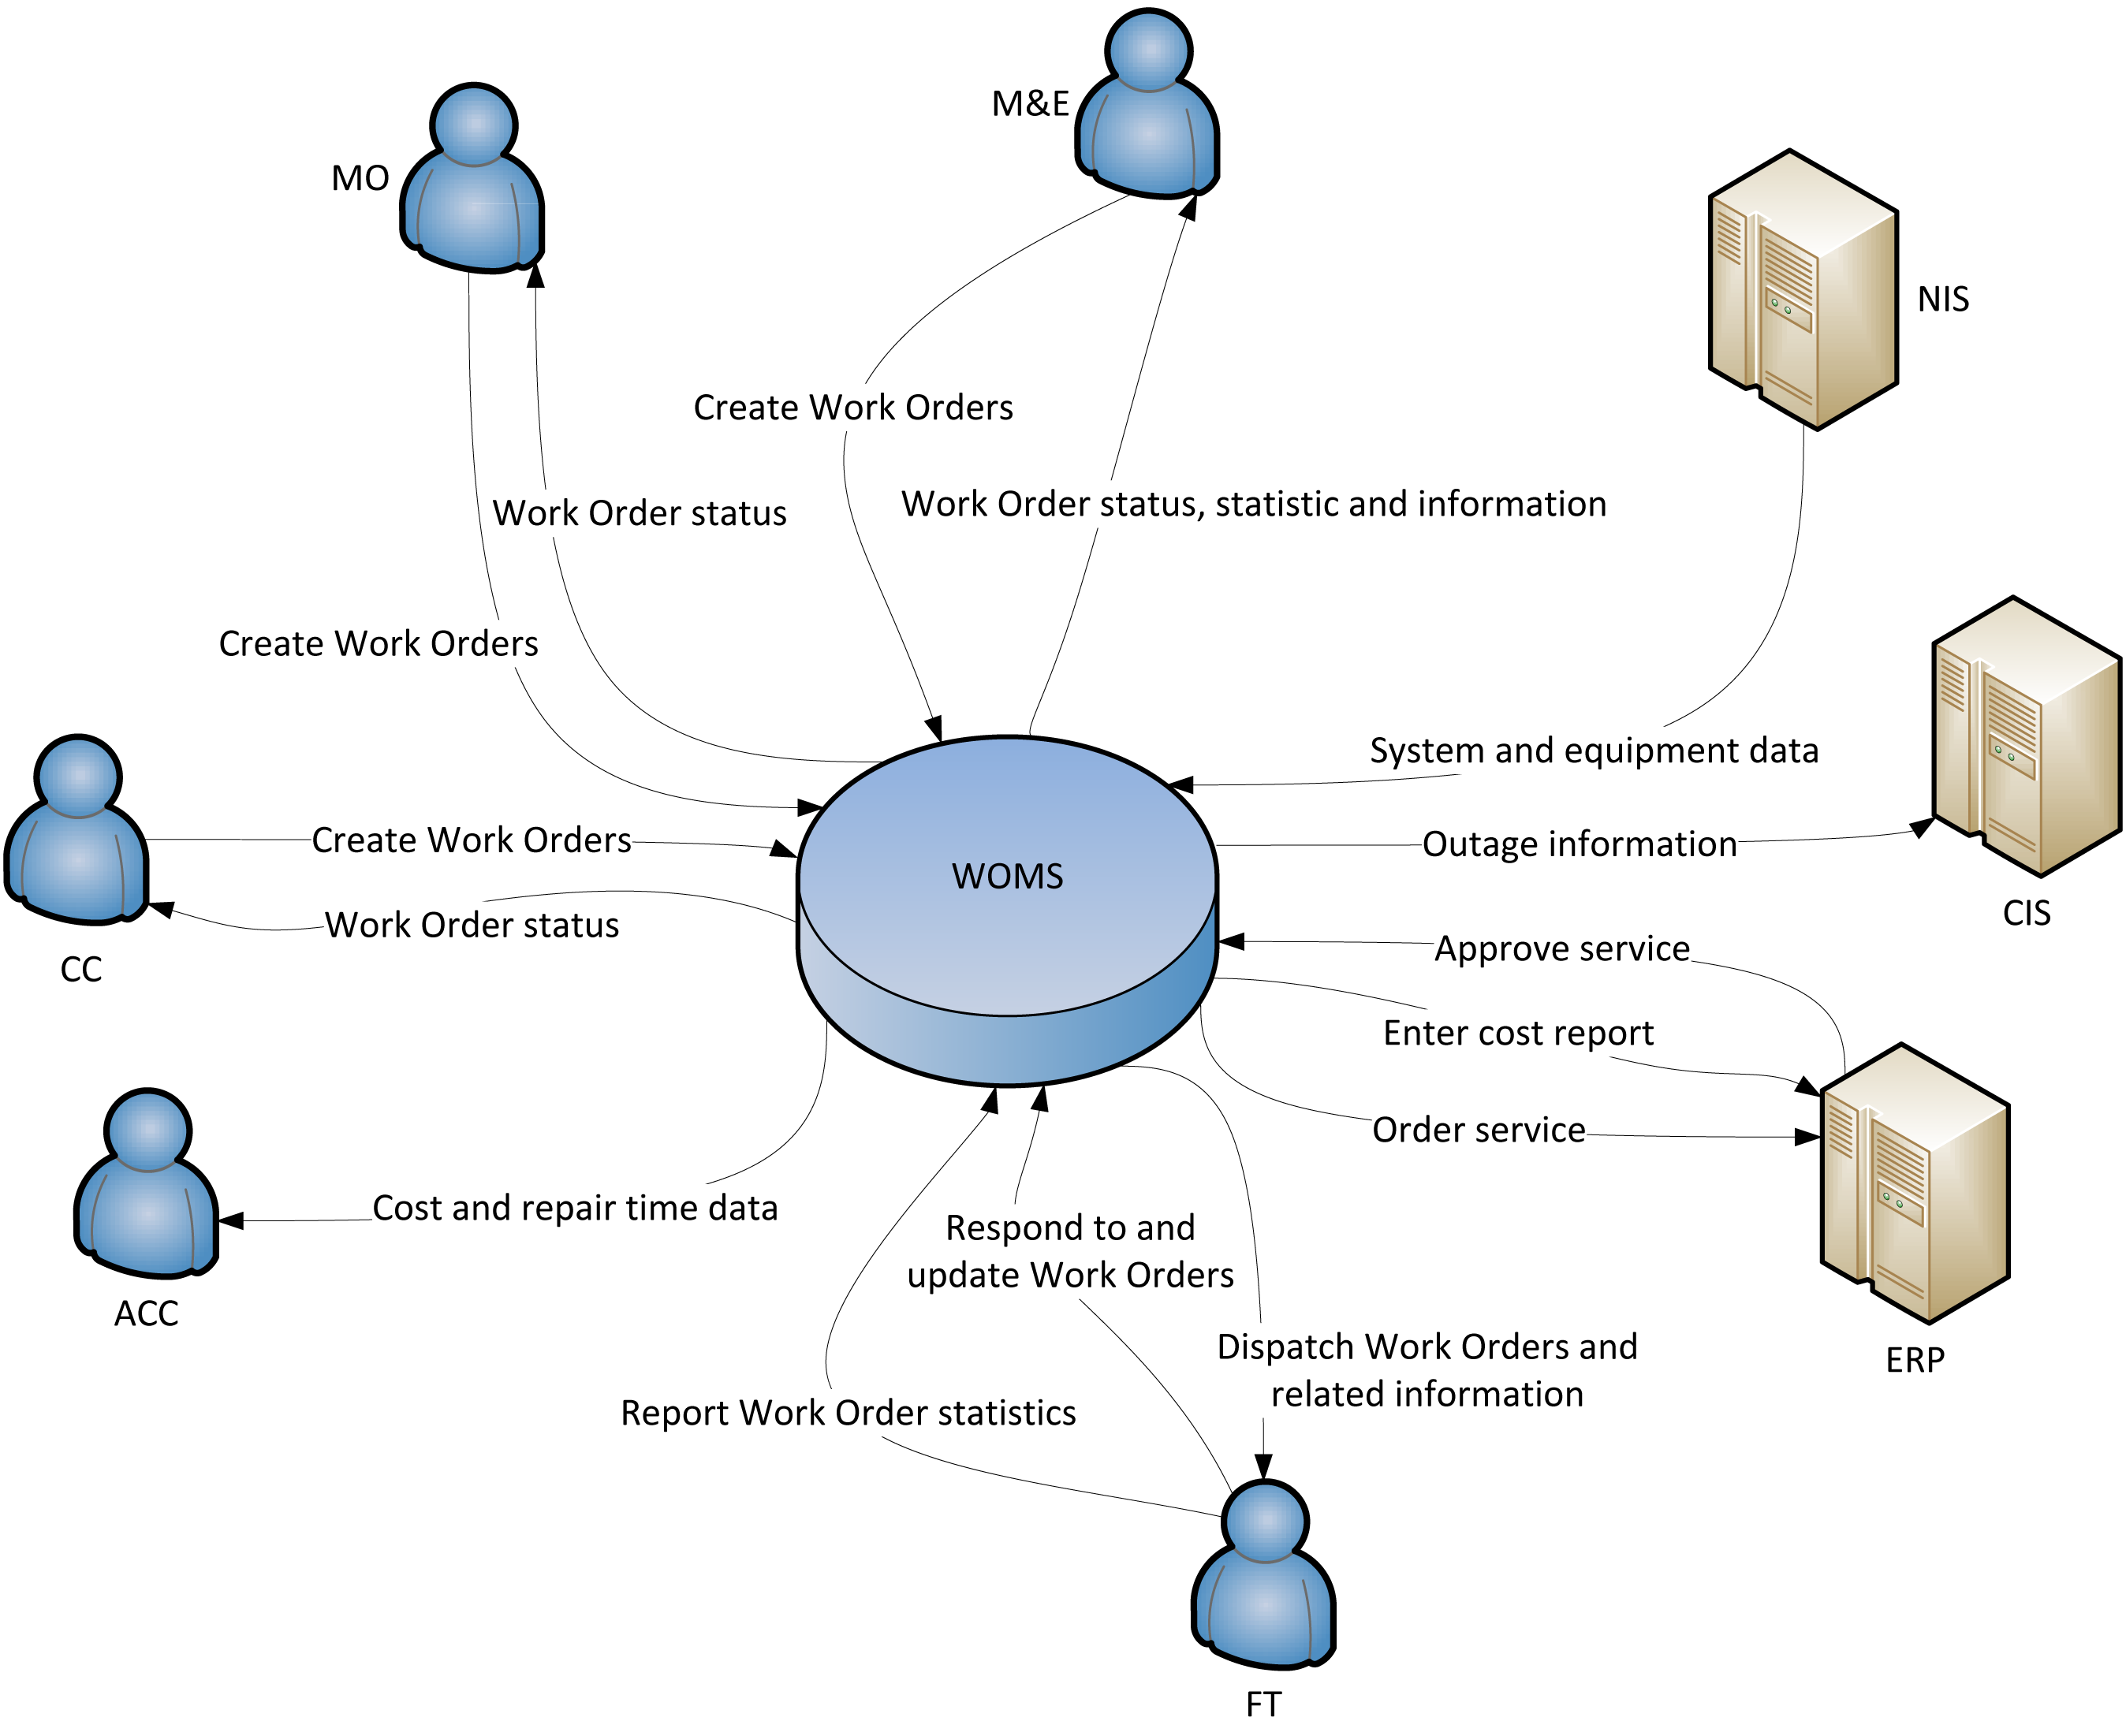
\includegraphics[scale = 0.9, angle = 90]{images/context_diagram.png}
	\label{appendix_a_context_diagram}
	\caption{Context Diagram}
\end{figure}

%\clearpage
 

\end{document}
